\subsection{Unittesten}
Voor het unit testen van de API is er gebruik gemaakt van xUnit (voor meer informatie zie sectie \ref{section:Bouwomgeving}).
Unit testen worden gebruikt om der verschillende logica van het systeem te testen.
Hierom zijn testen geschreven voor handlers en mappers in de applicatie.
Een voorbeeld van zo'n unit test is te zien in figuur \ref{fig:ExampleUnitTest}.
Verder is er een overzicht van de verschillende unittesten in figuur \ref{fig:OverviewUnitTests}.

\whitespace[2]
\begin{graphic}
	\captionsetup{type=figure}
	\caption{Geimplementeerde unit test}
	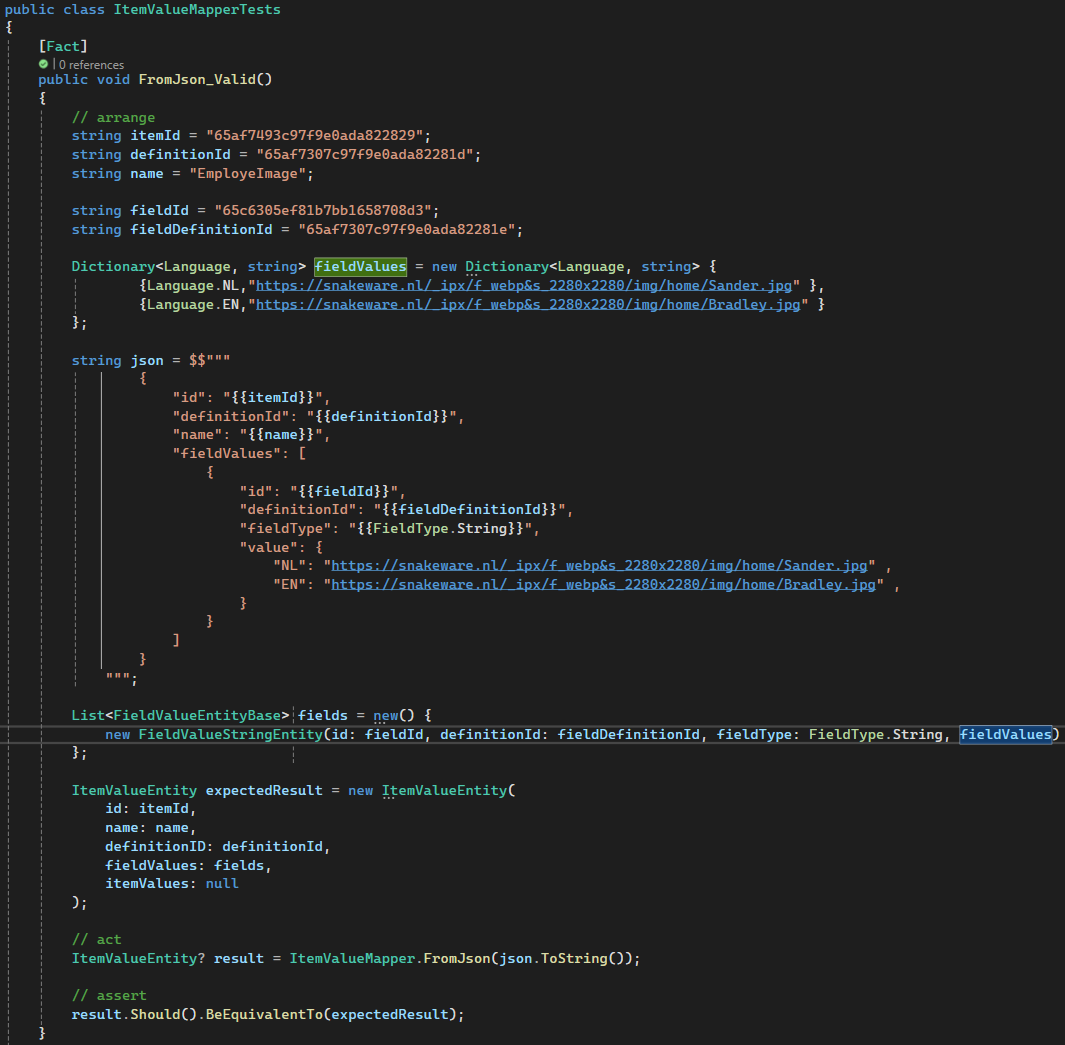
\includegraphics[scale=0.55]{ExampleUnitTest.png}
	\label{fig:ExampleUnitTest}
\end{graphic}
